%\documentclass[fleqn]{book}
\documentclass[11pt]{amsbook}

\usepackage[turkish]{babel}

%\usepackage{../HBSuerDemir}	% ------------------------
\usepackage{../Ceyhun}	% ------------------------
\usepackage{../amsTurkish}


\begin{document}
% ++++++++++++++++++++++++++++++++++++++
\hPage{008}
% ++++++++++++++++++++++++++++++++++++++

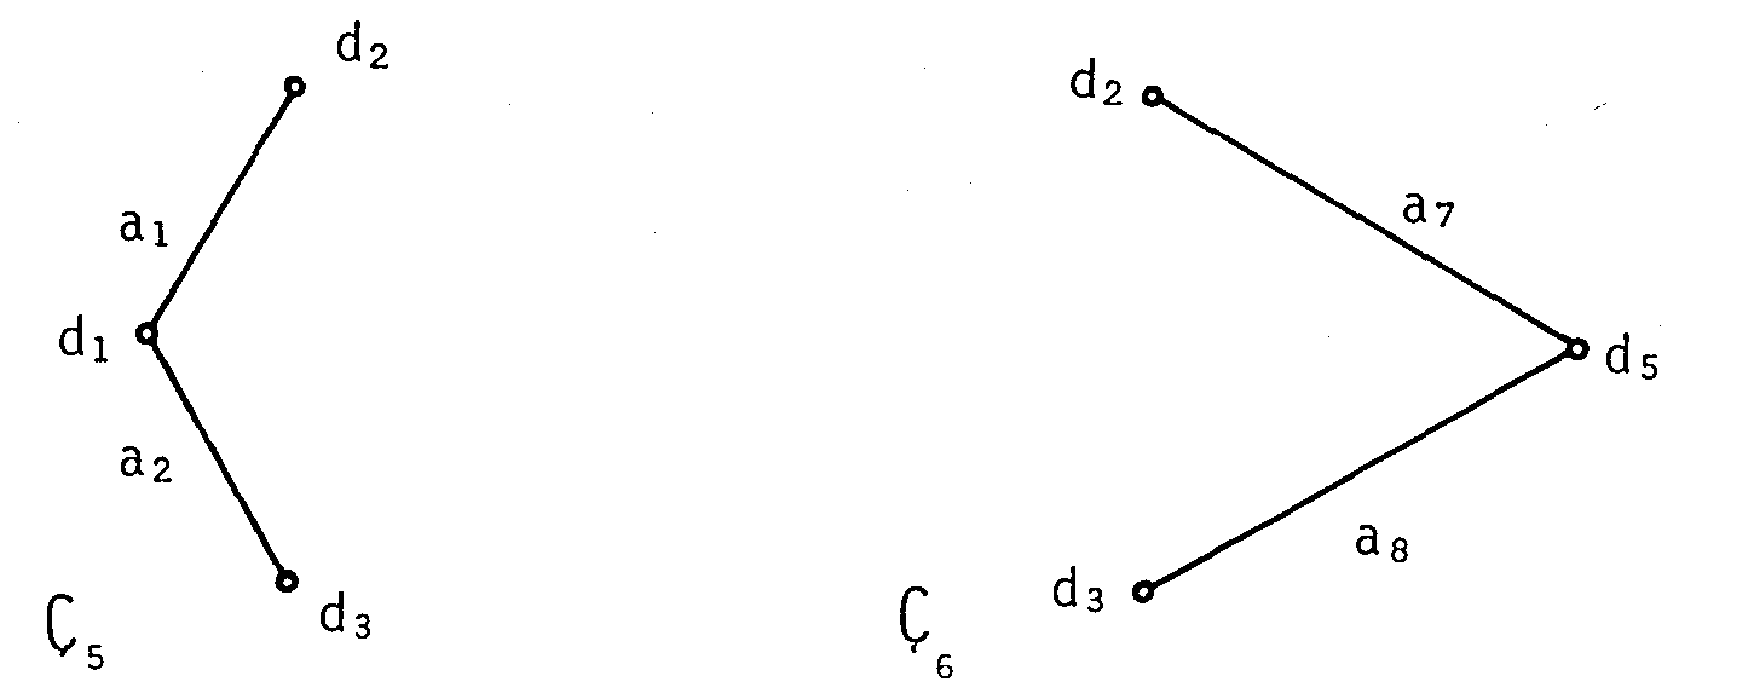
\includegraphics[width=\textwidth, height=6cm]{images/ceyhun-008-fig01}
    
\hspace{3cm} (ç) \hspace{9cm} (d)

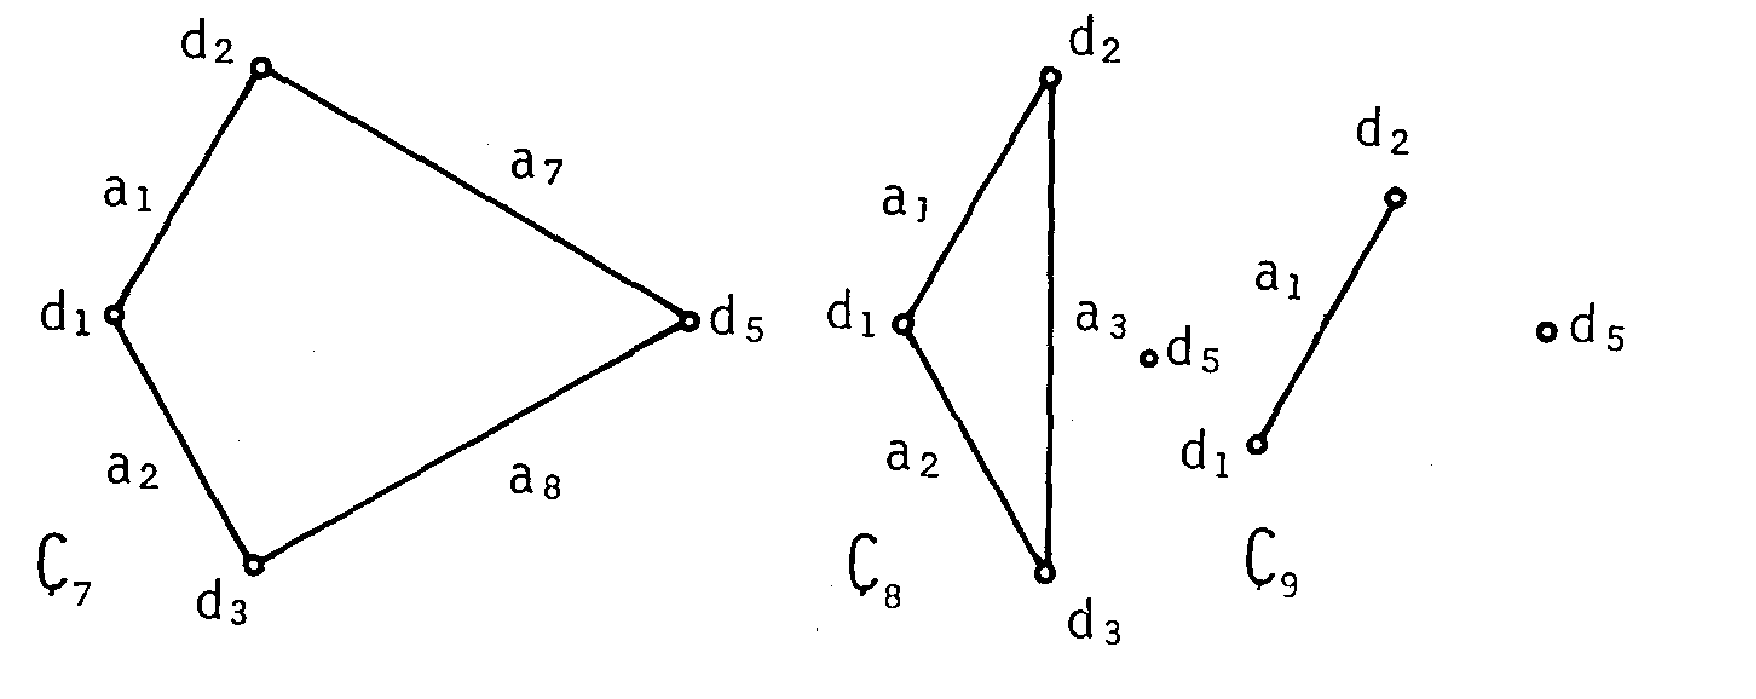
\includegraphics[width=\textwidth, height=6cm]{images/ceyhun-008-fig02}

\hspace{3cm} (e) \hspace{6cm} (f) \hspace{2cm} (g)

\figurename{ 1.1.6} $Ç_{1}\ ve\ Ç_{2}$ üzerine uygulanan işlemlerin\\
açıklanması. 

\hspace{3cm} $Ç_{3}=Ç_{1}\cup Ç_{2}$ \hspace{5cm} $Ç_{6}=Ç_{2}-Ç_{1}$\\

\hspace{3cm} $Ç_{4}=Ç_{1}\cap Ç_{2}$ \hspace{5cm} $Ç_{7}=Ç_{1}\textcircled{+}Ç_{2}$\\

\hspace{3cm} $Ç_{5}=Ç_{1}-Ç_{2}$ \hspace{5cm} $Ç_{8}=Ç_{1}-(d_{4})$\\


\begin{center}
    
    $Ç_{9}=Ç_{1}-(d_{3},d_{4})$
    
\end{center}

\end{document}